%-------------------------
%device-revisited.tex
%(c) H.Buchmann FHNW 2018
%export TEXINPUTS=${HOME}/fhnw/edu/:${HOME}/fhnw/edu/tinL/config/latex:${HOME}/fhnw/edu/config//:
%-------------------------
\documentclass{beamer}
\usepackage{latex/beamer}
%---------------------
%local defines
%(c) H.Buchmann FHNW 2009
%$Id$
%---------------------
\newcommand{\target} {\beaglebone\xspace}
\newcommand{\targetS}{{\bf BBG}\xspace}
\newcommand{\host}   {{\em Host}\xspace}
\newcommand{\targetroot} {{\bf target-root}\xspace}
\newcommand{\kernel} {{\bf kernel}\xspace}
\renewcommand{\c}{{\bf C}\xspace}
\newcommand{\cpp}{{\bf C++}\xspace}
\newcommand{\posix}{{\bf POSIX}\xspace}

\input{/home/buchmann/latex/dirtree/dirtree.tex}
\usepackage{svg}
\usepackage[absolute]{textpos}
\setlength{\TPHorizModule}{1mm}
\setlength{\TPVertModule}{1mm}

\begin{document}


\newcommand{\ksp}{{\em kernel-space}\xspace}
\newcommand{\usp}{{\em user-space}\xspace}
\newcommand{\hw}{{\em HW}\xspace}
\title[Hardwarwe]{Hardware}

\frame{\titlepage}

\begin{frame}{Um was geht es ?}{Hardware}
 \begin{itemize}
  \item \usp $\to$ \ksp $\to$ \hw
  \begin{itemize}
   \item via  {\em sysfs}
  \end{itemize}
  \item \hw $\to$  \ksp $\to$ \usp
  \begin{itemize}
   \item Interrupts
  \end{itemize}  
 \end{itemize}
\end{frame}

\begin{frame}{Unsere Hardware}
\begin{center}
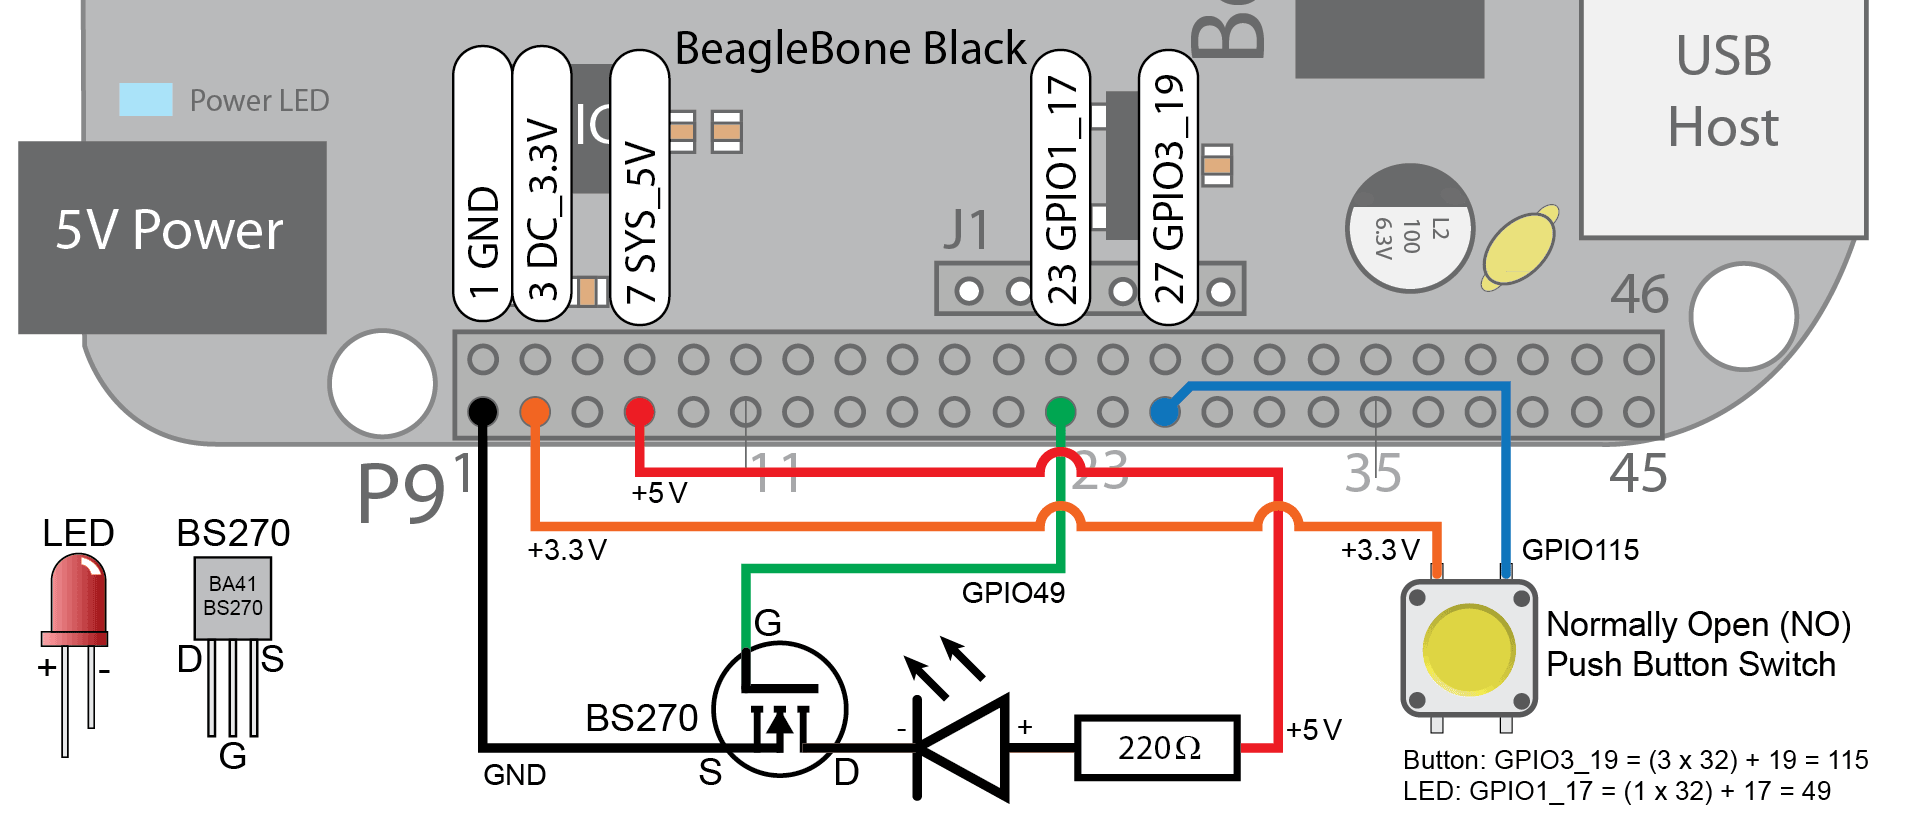
\includegraphics[width=0.875\textwidth]{Button-and-LED-large.png}
\end{center}
{\tiny \copyright \url[http]{derekmolloy.ie/kernel-gpio-programming-buttons-and-leds}}
\end{frame}

\part{\usp}
\frame{\partpage}
\begin{frame}{Vom \usp aus}{In Verzeichnis \cod{/sys/class/gpio}}
\begin{itemize}
 \item Output \cod{gpio49}
 \begin{itemize}
 \item \cod{cd gpio49}
 \item \cod{echo out > direction}
 \item \cod{echo 1 > value} \cod{echo 0 > value}
 \end{itemize}
 \item Input \cod{gpio115}
 \begin{itemize}
  \item entsprechend
 \end{itemize} 
\end{itemize}
\end{frame}

\begin{frame}{Aufgabe}{Skript}
 \begin{itemize}
  \item blink
  \item Polling
  \begin{itemize}
   \item read switch set led
  \end{itemize}
 \end{itemize}
\end{frame}


\part{LKM}
\frame{\partpage}
\section{linux/gpio.h}
\begin{frame}{Loadable Kernel Module (LKM)}{\cod{gpio-0.c}}
 \begin{itemize}
  \item eigenes Verzeichnis in  \cod{sys}: \cod{my-hw}
  \item einen File \cod{led} mit \cod{rw}:
  \begin{itemize}
   \item write: \cod{echo {\em x}> /sys/my-hw/led}
   \begin{description}[x=t$|$T]
    \item[x=1] set led
    \item[x=0] clear led
    \item[x=t$|$T] toggle led
   \end{description} 
   andere Werte von \cod{x} �ndern nichts
   \item read: \cod{cat /sys/my-hw/led}
   \begin{description}
    \item [1] led on
    \item [0] led off
   \end{description} 
  \end{itemize} 
 \end{itemize}
\end{frame}

\begin{frame}{Was Sie brauchen}{Pin 49 ist Output}
\begin{itemize}
 \item  \href{https://elixir.bootlin.com/linux/latest/source/include/linux/gpio.h\#L115}
             {\cod{gpio\_request}}
 \item  \href{https://elixir.bootlin.com/linux/latest/source/include/linux/gpio.h\#L131}
             {\cod{gpio\_free}}
 \item  \href{https://elixir.bootlin.com/linux/latest/source/include/linux/gpio.h\#L152}
             {\cod{gpio\_direction\_output}}
 \item \href{https://elixir.bootlin.com/linux/latest/source/include/linux/gpio.h\#L169} 
             {\cod{gpio\_set\_value}}            
\end{itemize}     
\end{frame}

\section{Direkt GPIO}
\begin{frame}{Direkter Zugriff auf die \hw}
 \begin{itemize}
  \item die Register
  \item als Memory
  \item Siehe \cod{src/gpio.h}
 \end{itemize}
\end{frame}

\begin{frame}{Informationen}
 \begin{itemize}
  \item \cod{cat /proc/iomem}
 \end{itemize}
\end{frame}


\begin{frame}{Register}{im Memory}
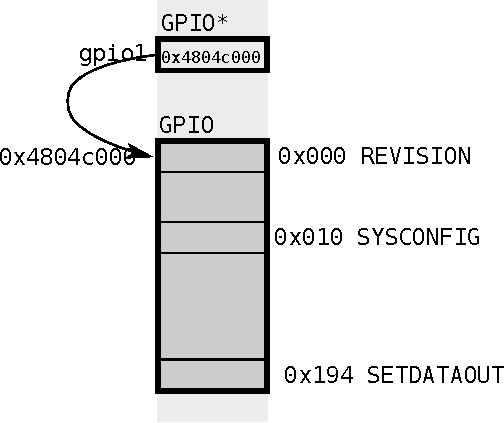
\includegraphics[height=0.75\textheight]{hw-gpio.pdf}
\begin{textblock}{100}(70,60)
\begin{itemize}
 \item \cod{GPIO* \_\_iomem  gpio1=???}
 \item \cod{gpio1=ioremap(0x4804c000,0x1000)}
\end{itemize}
\end{textblock}
\end{frame}

\begin{frame}{Die einzelnen Bits}{die Operationen}
 \begin{description}
  \item[setBit] Operation $|$
  \item[clrBit] Operation $\&$
 \end{description}
\end{frame}

\begin{frame}{Loadable Kernel Module (LKM)}{\cod{gpio-1.c}}
\begin{itemize}
 \item Manual \cod{spruh73l.pdf} Abschnitt 25
 \item \cod{gpio.h} die einzelnen Register:
 \begin{description}[CLEARDATAOUT]
  \item[REVSION] f�r Test
  \item[OE] OutputEnable
  \item[DATAIN] Data In
  \item[CLEARDATAOUT] L�scht Bit
  \item[SETDATAOUT] Setzt Bit
 \end{description}
 \item \href{https://elixir.bootlin.com/linux/latest/source/arch/alpha/include/asm/io.h\#L286}
            {\cod{ioremap}}
 \item \href{https://elixir.bootlin.com/linux/latest/source/arch/alpha/include/asm/io.h\#L306}
            {\cod{iounmap}}
\end{itemize}
\end{frame}

\section{Interrupt}
\begin{frame}{Outline}
 \begin{description}
  \item[Callback] Hollywood Prizip: 
   \begin{quote}
    don't call us, we'll call you.
   \end{quote}
   \vspace{-7mm}
   \begin{itemize}
    \item die Hardware ruft zur�ck
   \end{itemize}
  \item[Interrupts] Der Schritt zur Echtzeit
  \begin{itemize}
   \item Die Hardware ruft Software auf
   \item Elementare Anwendung vom {\em callback}
   \item Ereignisgesteuert: {\em event driven}
  \end{itemize}
 \end{description}
\end{frame}

\begin{frame}{SW braucht HW}{und umgekehrt}
\begin{center}
 
\includegraphics[width=0.75\textwidth]{hw-sw-calls.pdf}
\end{center}
 \begin{block}{Beispiel}
  \begin{description}
   \item[SW$\to$HW]
    \begin{itemize}
     \item Setze LED
     \item Schreibe Buchstabe 
    \end{itemize}
    \item[HW$\to$SW]
     \begin{itemize}
      \item Ein {\em timer} tick
      \item Tastatur Taste gedr�ckt
     \end{itemize}
  \end{description}
 \end{block}
 \vspace{-5mm}
 \remark{Beide Richtungen {\em SW$\to$HW} und {\em HW$\to$SW} sind wichtig}
\end{frame}

\begin{frame}{Asynchron}{jederzeit}
\begin{block}{Normale Programmausf�hrung: Thread}
\begin{center}
 
\includegraphics[width=0.5\textwidth]{thread.pdf}
\end{center}
\end{block}
\vspace{-5mm}
\begin{block}{Interrupt}
 \vspace{-5mm}
  \begin{center}
 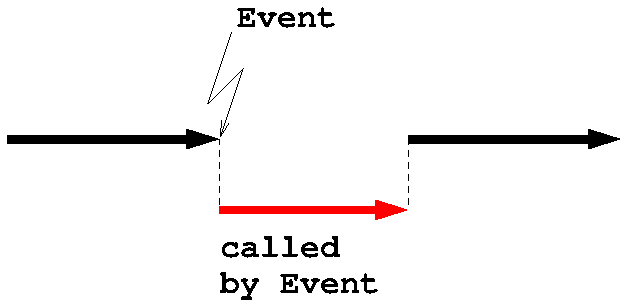
\includegraphics[width=0.5\textwidth]{interrupted-thread.pdf}
 \end{center}
\end{block} 
\vspace{-5mm}
\begin{description}[unsichtbar]
 \item[jederzeit] Zwischen zwei Instruktionen
 \item[unsichtbar] vom Thread aus gesehen
\end{description}
\end{frame}

\begin{frame}{Informationen}
 \begin{itemize}
  \item \cod{cat /proc/interrupts}
 \end{itemize}
\end{frame}

\subsection{gpio-2.c}
\begin{frame}{Ziel}
 \begin{itemize}
  \item Interrupt erkennen
  \item Switch
  \begin{itemize}
   \item dr�cken: erzeugt interrupt: \cod{IRQF\_TRIGGER\_RISING}
   \item loslassen: erzeugt interrupt:\cod{IRQF\_TRIGGER\_FALLING}
  \end{itemize}
 \end{itemize}
\end{frame}

\begin{frame}[fragile]{gpio-2.c}{schrittweise}
 \begin{itemize}
  \item \href{https://elixir.bootlin.com/linux/latest/source/include/linux/gpio.h\#L147}
             {\cod{gpio\_direction\_input}}
  \item \href{https://elixir.bootlin.com/linux/latest/source/include/linux/gpio.h\#L216}
             {\cod{gpio\_to\_irq}}
  \item \href{https://elixir.bootlin.com/linux/latest/source/include/linux/interrupt.h\#L146}
             {\cod{request\_irq}}    
 \end{itemize}
 \begin{block}{Der Handler}
\begin{lstlisting}
static  irqreturn_t onSWI(int id,void* d)
{
 printk("onSWI\n"); /* debug */
 /* do something */
 return IRQ_HANDLED;
}
\end{lstlisting}
 \end{block}
\end{frame}


\section{Tasklet}

\begin{frame}{foreground-background}{Tasklet:die Verbindung}
 \begin{description}
  \item[foreground] der/die Interrupts
  \item[background] die normale Ausf�hrung
  \item[tasklet] Verbindung \cod{foreground} $\to$ \cod{background}
 \end{description}
\end{frame}

\begin{frame}{Tasklet}{foreground $\to$ background}
\begin{center}
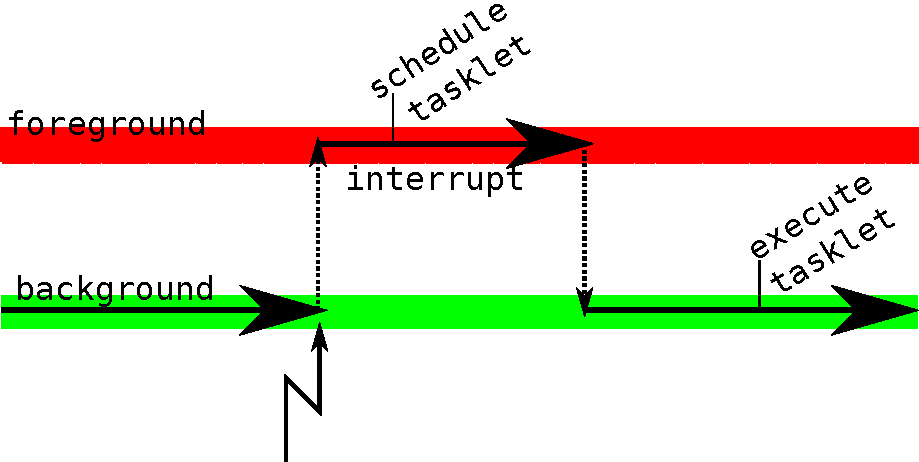
\includegraphics[width=10cm]{tasklet.pdf}
\end{center}
\end{frame}

\subsection{gpio-3.c}
\begin{frame}[fragile]{gpio-3.c}{schrittweise}
 \begin{itemize}
  \item Definition global 
       \href{https://elixir.bootlin.com/linux/latest/source/include/linux/interrupt.h\#L537}
            {\cod{tasklet\_struct}}
  \item Initialisation
       \href{https://elixir.bootlin.com/linux/latest/source/include/linux/interrupt.h\#L618}
            {\cod{tasklet\_init}}
  \item Scheduling im {\em foreground}
        \href{https://elixir.bootlin.com/linux/latest/source/include/linux/interrupt.h\#L583}
            {\cod{tasklet\_schedule}}
 \end{itemize}
 \begin{block}{Der Handler}
 \begin{lstlisting}
/* *not* called in interrupt */
static void onSWITasklet(unsigned long data)     
{
 /* do something */  
}
 \end{lstlisting}
 \end{block}
\end{frame}



\part{\ksp $\to$ \usp\\Semaphore \& Co.}
\title{\ksp $\to$ \usp}
\frame{\partpage}
\section{Semaphore}

\begin{frame}{Semaphore}
\begin{columns}
\begin{column}{0.5\textwidth}
\includegraphics[height=0.5\textheight,angle=-90]{BhfEpfenhofen_Ausfahrsignale_Talaufwaerts_II.JPG}

{\tiny \copyright 
\url{upload.wikimedia.org/wikipedia/commons/0/0b/BhfEpfenhofen\_Ausfahrsignale\_Talaufwaerts\_II.JPG}}
\end{column}
\begin{column}{0.5\textwidth}
 \begin{itemize}
  \item \cod{down}: Signal zu
  \begin{itemize}
   \item warten
  \end{itemize}
  \item \cod{up}: Signal offen
  \begin{itemize}
   \item fahren
  \end{itemize}
 \end{itemize}
\end{column}
\end{columns}
\end{frame}

\begin{frame}{Tasklet-Semaphore}
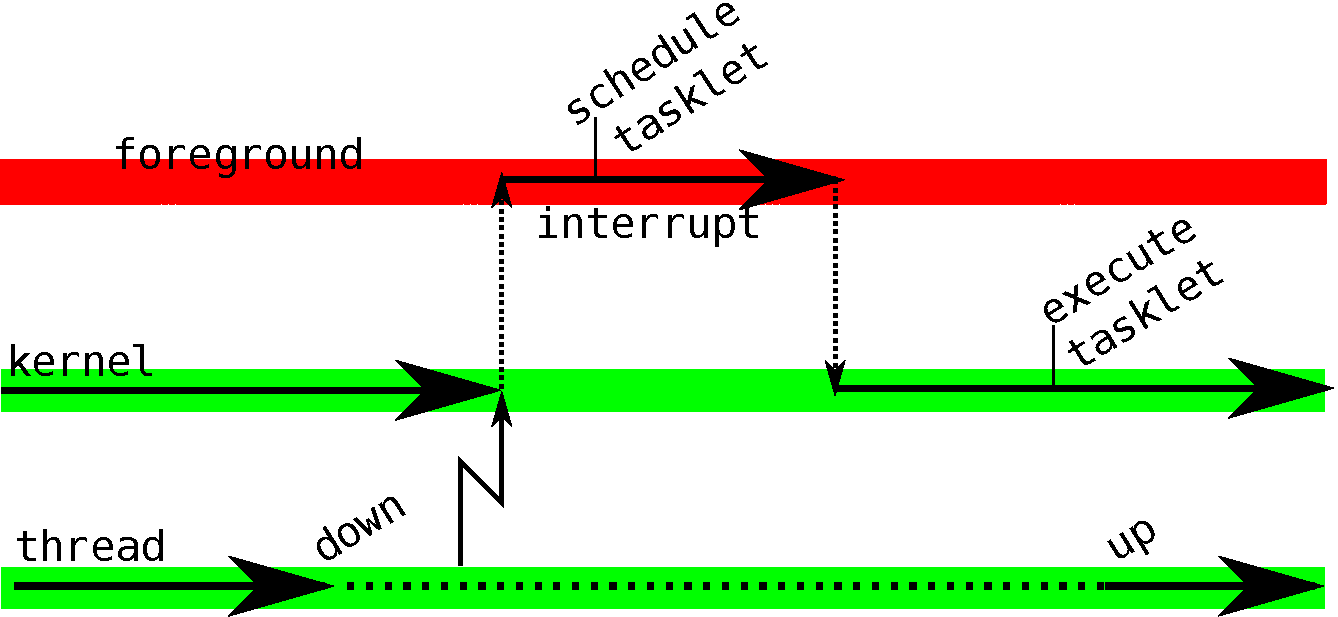
\includegraphics[width=10cm]{tasklet-semaphore.pdf}
\end{frame}

\subsection{gpio-4.c}

\begin{frame}{gpio-4.c}{schrittweise}
 \begin{itemize}
  \item Definition global 
     \href{https://elixir.bootlin.com/linux/latest/source/include/linux/semaphore.h\#L16}
          {\cod{semaphore}}
  \item Initialisation
  
   \href{https://elixir.bootlin.com/linux/latest/source/include/linux/semaphore.h\#L32}
        {\cod{sema\_init}} anfangs geschlossen 
  \item Im Tasklet
   \href{https://elixir.bootlin.com/linux/latest/source/include/linux/semaphore.h\#L44}
        {\cod{up}}: �ffne
  \item Im \cod{get\_swi}
   \href{https://elixir.bootlin.com/linux/latest/source/include/linux/semaphore.h\#L39}
        {\cod{down}}: warte \& schliesse
 \end{itemize}
\end{frame}

\section{Wait-Queue}

\begin{frame}{Wait queue}{Task/processe warten}
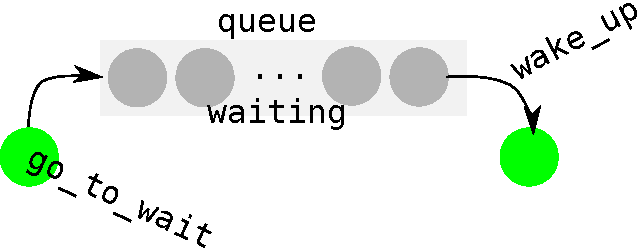
\includegraphics{queue.pdf}

\vspace{5mm}

\includegraphics[width=0.25\textwidth]{queue-legend.pdf}
\end{frame}

\subsection{gpio-5.c}
\begin{frame}{gpio-5.c}{schrittweise}
 \begin{itemize}
  \item Definition global
  \begin{itemize}
   \item \href{https://elixir.bootlin.com/linux/latest/source/include/linux/wait.h\#L34}
              {\cod{wait\_queue\_head}}
   \item \cod{swiN} die Anzahl Schaltungen von \cod{swi}
  \end{itemize}
  \item go to wait
  \begin{itemize}
   \item  \href{https://elixir.bootlin.com/linux/latest/source/include/linux/wait.h\#L442}
               {\cod{wait\_event\_interruptible}}
  \end{itemize}
  \item wakeup
  \begin{itemize}
    \item \href{https://elixir.bootlin.com/linux/latest/source/include/linux/wait.h\#L201}
               {\cod{wake\_up\_interruptible}}
  \end{itemize}
 \end{itemize}
\end{frame}

\section{Semaphore-Queue}

\begin{frame}{Mit eigener {\em Semaphhore-queue}}
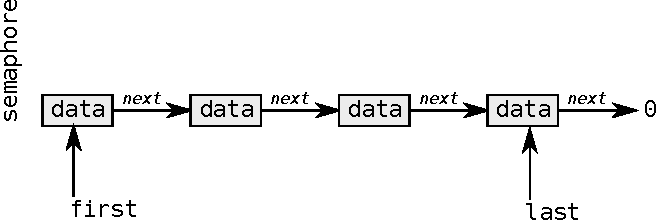
\includegraphics{semaphore-queue.pdf}
\vspace{-5mm}
\begin{itemize}
 \item put
  \begin{itemize}
   \item f�ge hinten an \cod{put}: data: Zustand des Schalters: \cod{on$|$off}
   \item �ffne Semaphore
  \end{itemize}
 \item get
 \begin{itemize}
  \item warte am Semaphore
  \item hole \cod{get} 
 \end{itemize}
\end{itemize}
\end{frame}


\subsection{Simply Linked List}
\begin{frame}{Die {\em Queue}}{einfach verlinkte Liste}
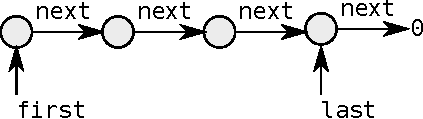
\includegraphics{queue-generic.pdf}
\end{frame}


\begin{frame}{Die {\em Queue}}{put}
\begin{block}{before}
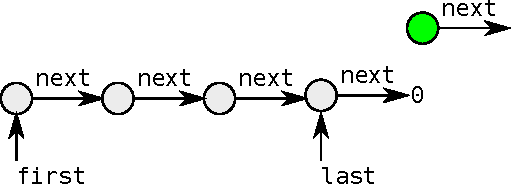
\includegraphics{put-before.pdf}
\end{block}
\begin{block}{after}
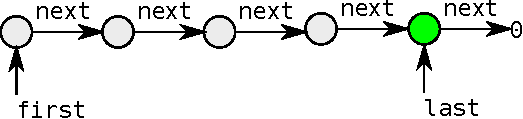
\includegraphics{put-after.pdf}
\end{block}
\end{frame}

\begin{frame}{Die {\em Queue}}{get}
\begin{block}{before}
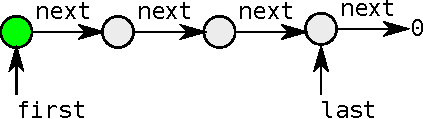
\includegraphics{get-before.pdf}
\end{block}
\begin{block}{after}
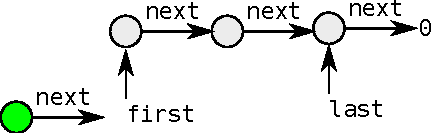
\includegraphics{get-after.pdf}
\end{block}
\end{frame}

\subsection{queue.c}

\begin{frame}{Verlinkte Listen}{Kommen immer wieder vor}
\begin{itemize}
 \item im userspace
 \item \cod{struct}
 \item \cod{init\_} 
 \item \cod{put\_}
 \item \cod{get\_}
  \item Dynamisches Memory
  \begin{itemize}
   \item  \cod{malloc}
   \item \cod{free}
  \end{itemize}
\end{itemize}
\end{frame}

\subsection{gpio-6.c}

\begin{frame}{Die Semaphore-Queue}
 \begin{itemize}
  \item \cod{struct} f�r Semaphore-Queue
  \item \cod{init\_} 
  \item \cod{put\_}
  \item \cod{get\_}
  \item Dynamisches Memory
  \begin{itemize}
   \item  \cod{kmalloc}
   \item \cod{kfree}
  \end{itemize}
 \end{itemize}
\end{frame}

\begin{frame}[fragile]{TODO's}{Im Zusammenhang mit den Interrups}
 \begin{itemize}
  \item mehr Informationen in \cod{buf} von \cod{get\_swi} zur�ckgeben: 
  \begin{lstlisting}
  struct SWIInfo
  {
   time_t   when;
   unsigned nbr;  //the number of switching
   unsigned state; //on|off
  };
  \end{lstlisting}
 \item Queue als {\em ringbuffer}
 \end{itemize}
\end{frame}

\subsection{TODO Mehr Info:gpio-8.c}

\begin{frame}{\cpp gemacht mit \c}
 \begin{itemize}
  \item \cod{src/queue-a-la-cpp.c}
 \end{itemize}
\end{frame}

\begin{frame}[fragile]{SWIInfo}
\begin{lstlisting}
typedef struct SWIInfo
{
 time_t       when;
 unsigned     nbr;
 unsigned     state;
} SWIInfo;
\end{lstlisting}
\begin{itemize}
 \item Die Zeit
 \begin{itemize}
  \item Globale Variable: \cod{jiffies}
 \end{itemize}
\end{itemize}
\end{frame}

\begin{frame}{gpio-8.c}{Vorgehen}
 \begin{itemize}
  \item \cod{currentE} 
  \begin{itemize}
   \item der aktuelle Eintrag: gesetzt von \cod{onSWI}
  \end{itemize}
  \item tasklet \cod{call-back}
  \begin{itemize}
   \item {\bf kopiert} \cod{currentE} in den Ringbuffer: \cod{put}
  \end{itemize}
  \item \cod{get\_swi}
  \begin{itemize}
   \item {\bf kopiert} vom Ringbuffer in den \cod{buf}:\cod{get}
  \end{itemize}
 \end{itemize}
\end{frame}


\section{Semaphore-Ringbuffer}

\begin{frame}{Ringbuffer}
 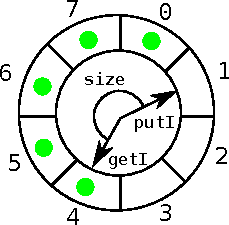
\includegraphics{ringbuffer.pdf}
 \begin{textblock}{100}(60,40)
 \begin{itemize}
  \item \cod{put}
  \item \cod{get}
  \item \C
  \begin{itemize}
   \item \cod{ring-buffer.c}
  \end{itemize}
  \item \CPP
  \begin{itemize}
   \item \cod{ring-buffer-cpp.cc}
  \end{itemize}
 \end{itemize}
 \end{textblock}
\end{frame}

\subsection{Ringbuffer}


\part{\usp\ \cpp}
\title{\usp\ \cpp}
\frame{\partpage}
\begin{frame}{{\em userspace} vs. {\em kernelspace}}{Systemcalls}
\begin{center}
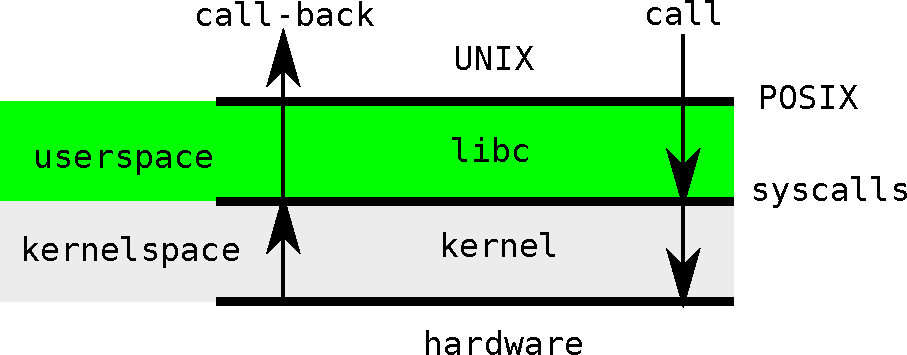
\includegraphics[width=10cm]{userspace-kernelspace.pdf}
\end{center}
\begin{description}[kernelspace]
 \item[userspace] geschützt, limitierte Zugriffsmöglichkeiten
 \item[kernelspace] ungeschützt, unlimitierte Zugriffsmöglichkeiten
\end{description}
\end{frame}

\subsection{syscalls}
\begin{frame}[fragile]{Syscall aus {\em user} Sicht }{\src{syscall-c.c}}
 \begin{lstlisting}[basicstyle=\footnotesize]
 /* write(f,void* buffer,unsigned len) */
 char s[]="Hello World\n";
         /*01234567890 */
 syscall(4,0,s,12);  /* we are in userspace */
     /*  |------------------ code for write */
 \end{lstlisting}
\end{frame}

\begin{frame}{Verzeichnisstruktur}
\dirtree{%
.1 25-modules.
.2 config.
.2 tc \DTcomment{link to toolchain}.
.2 target \DTcomment{sshfs \targetS}.
.2 work.
}
\remark{Siehe auch 17-build}
\end{frame}

\subsection{Aufgaben}
\begin{frame}{Aufgaben}
 \begin{itemize}
  \item Systemcall für \host/\targetS mit \c und \cpp
 \end{itemize}
\end{frame}


\end{document}
